\section{ModelVM Architecture \& Runtime Abstraction}
\label{sec:runtime_architecture}

Executing complex multi-disciplinary language model workloads on resource-constrained consumer hardware requires resolving a core contradiction: domain-specialized open-weight models deliver superior accuracy on targeted technical tasks compared to monolithic generalists, but their collective memory footprint ($M_{\text{active,total}} = 52.7\,\text{GB}$) far exceeds commodity memory envelopes ($\mathcal{B}_{\text{RAM}} = 8.0\,\text{GB}$). To resolve this bottleneck without sacrificing specialization or state integrity, ModelVM introduces an operating-system-inspired runtime architecture. 

In this section, we present the structural foundations of ModelVM. We first de-center the operating system metaphor, establishing the precise theoretical and practical boundaries between classical virtual memory and cognitive runtime virtualization. We then detail the architectural flow and subsystem coordination governing the Cognitive Kernel, Model Pager, and Cognitive Scheduler. Finally, we formulate the residency state and provide an inductive proof of the runtime memory invariant, characterizing its relationship to physical host and accelerator memory headroom.

\subsection{De-centering the OS Metaphor}
\label{sec:os_analogy}

The conceptual lineage of ModelVM traces directly to Peter Denning's foundational work on virtual memory and working-set dynamics~\cite{denning1968working}. In early mainframe computing, programmers encountered a physical constraint analogous to today's LLM deployment barrier: individual software systems required more primary magnetic core memory than was physically installed. Classical virtual memory resolved this disparity by decoupling the logical address space referenced by software processes from the physical page frames provided by hardware, transparently swapping unreferenced pages to secondary disk storage.

While this paradigm inspires our design, we explicitly decouple ModelVM from literal kernel-level mechanisms to avoid false equivalence. Table~\ref{tab:os_analogy} formalizes the conceptual correspondence while delineating critical systems differences.

\begin{table*}[t]
\small
\centering
\caption{System Mapping: Classical Operating System Virtual Memory vs.\ ModelVM Runtime Abstraction}
\label{tab:os_analogy}
\setlength{\tabcolsep}{4pt}
\renewcommand{\arraystretch}{1.18}
\begin{tabular}{>{\RaggedRight\bfseries}p{2.85cm} >{\RaggedRight}p{3.55cm} >{\RaggedRight}p{3.78cm} >{\RaggedRight}p{5.20cm}}
\toprule
\textbf{Systems Dimension} & \textbf{Classical OS}\newline\textbf{Virtual Memory} & \textbf{ModelVM Runtime}\newline\textbf{Abstraction} & \textbf{Architectural Distinction} \\
\midrule
Execution Unit & Operating System Process & Domain Capability Stage ($s_t$) & Coarse procedural step vs.\ machine instruction stream \\
\addlinespace[3.5pt]
Execution Engine & Physical Hardware CPU\,/\,Core & Heterogeneous Specialist Model ($M_t$) & Neural network parameter logic executing on host/device \\
\addlinespace[3.5pt]
State Abstraction & Process Control Block (PCB) \& Virtual Address Space & Cognitive State Packet ($\mathcal{S}_t$) & Structured typed 9-tuple semantic carrier vs.\ raw uninterpreted bytes \\
\addlinespace[3.5pt]
Memory\newline Allocation & Fixed-size Page Frames (4\,KB\,/\,2\,MB) & Model Weight Parameter Allocations ($\text{RAM}_{\text{req}}(m)$) & Multi-gigabyte tensor buffers vs.\ uniform hardware page frames \\
\addlinespace[3.5pt]
Primary Memory & Physical Host RAM & Active Execution Budget ($\mathcal{B}_{\text{RAM}}$, nominal $8.0\,\text{GB}$) & User-space configured quota vs.\ physical silicon capacity \\
\addlinespace[3.5pt]
Backing Store & Secondary Disk\,/\,Swap Partition & Serialized Model Catalog on NVMe ($\mathcal{B}_{\text{disk}} = 64.0\,\text{GB}$) & Structured parameter \mbox{safetensors\,/\,GGUF} vs.\ raw swap blocks \\
\addlinespace[3.5pt]
Fault Mechanism & Hardware Page Fault (MMU Interrupt) & Model Cache Miss (Runtime Interception) & Software-level stage routing vs.\ ring-0 exception handler \\
\addlinespace[3.5pt]
Residency\newline Tracking & Inverted Page Table\,/\,TLB & Resident Model Tracking Table ($\mathcal{R}_t$) & Object registry with access timestamps vs.\ hardware translation tables \\
\addlinespace[3.5pt]
Working Set & Past-window Page Frequency $W(t, \Delta)$ & Predictive Working Set $W(t, k)$ & Forward-looking task DAG lookahead vs.\ backward-looking sliding window \\
\addlinespace[3.5pt]
Context Switch & Register save/restore + address space swap & Typed CSP Handoff across Model Boundaries & Architecture-agnostic state merge vs.\ hardware thread context dump \\
\bottomrule
\end{tabular}
\end{table*}

\paragraph{Scope Boundaries and What ModelVM Is Not.}
To ensure scientific clarity, we define three explicit boundaries governing our abstraction:
\begin{enumerate}
    \item \textbf{Language Models are Processes, Not CPUs:} In classical systems, the CPU is the physical executor, while processes represent scheduled programs. In ModelVM, the physical host CPU and GPU accelerator remain the execution hardware. An open-weight language model is a specialized computational process containing frozen parameter weights that executes a cognitive transformation stage. ModelVM treats the model itself as the pageable computational resource.
    \item \textbf{User-Space Runtime, Not Ring-0 Kernel:} ModelVM does not modify kernel-level memory management units (MMUs), modify OS page tables, or install custom device drivers. It is a user-space systems runtime and execution middleware that coordinates weight streaming, inference dispatch, and state tracking.
    \item \textbf{Semantic State vs.\ Byte Buffers:} Classical operating systems are semantically agnostic; a page frame contains uninterpreted binary data. In contrast, language model handoffs require semantic state preservation. Swapping model weights alone is insufficient if the intermediate reasoning state is corrupted. ModelVM couples physical weight residency management with semantic state virtualization, ensuring that state transitions across heterogeneous architectures remain structured and architecture-agnostic.
\end{enumerate}

\subsection{Architectural Flow \& Subsystem Coordination}
\label{sec:subsystem_coordination}

The ModelVM architecture is organized into three tightly coupled subsystems coordinated by a centralized supervisory control path: the \textbf{Cognitive Kernel}, the \textbf{Model Pager}, and the \textbf{Cognitive Scheduler}. Figure~\ref{fig:modelvm_architecture} illustrates the architectural topology and dataflow pathways.

\begin{figure*}[t]
\centering
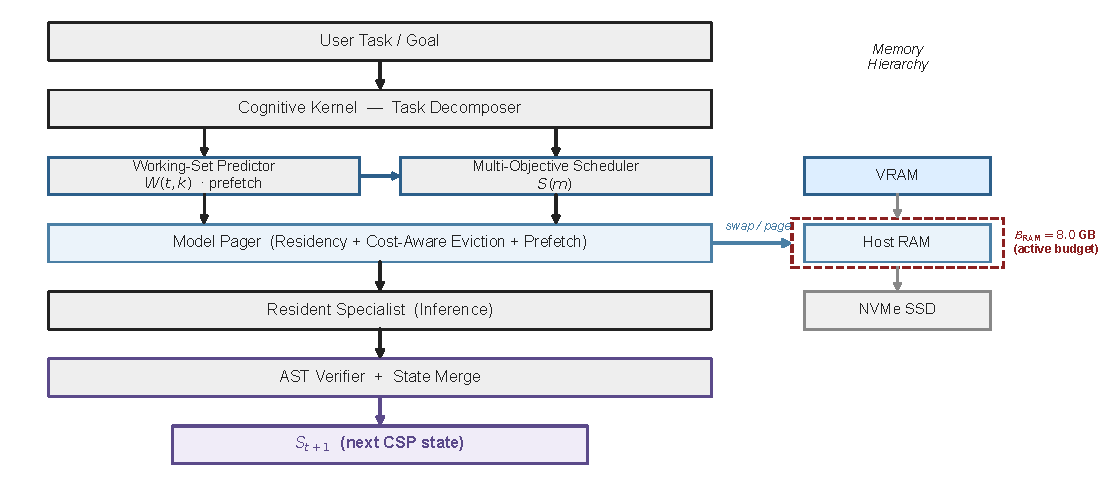
\includegraphics[width=\textwidth]{fig1_architecture.pdf}
\caption{ModelVM Architectural Topology (Class B full-width). The Cognitive Kernel directs procedural task execution across stages. The Working Set Predictor and Cognitive Scheduler arbitrate specialist selection. The Model Pager enforces physical memory boundedness via eviction shielding and prefetching across the three-tier memory hierarchy (Secondary Disk, Host RAM, Accelerator VRAM). The Inference Backend executes specialist transformations validated by an independent AST verifier.}
\label{fig:modelvm_architecture}
\end{figure*}

\paragraph{1. The Cognitive Kernel (\texttt{CognitiveKernel}).}
The Cognitive Kernel serves as the supervisory coordinator of the runtime:
\begin{itemize}
    \item \textbf{Procedural Decomposition:} Given a high-level task goal $G \in \Sigma^*$, the kernel invokes \texttt{TaskDecomposer} to produce an ordered sequence of $N$ dependent capability stages $S = [s_0, s_1, \dots, s_{N-1}]$, where each stage $s_t$ defines capability requirement $C(s_t) \in \mathcal{C}$ and domain instruction $\tau_t$.
    \item \textbf{State Virtualization Lifecycle:} The kernel instantiates the root state carrier $\mathcal{S}_0 = \langle G, \emptyset, \emptyset, \emptyset, \emptyset, \emptyset, \emptyset, \emptyset, \emptyset \rangle$ and threads it across stage boundaries. At each transition, the kernel merges validated updates $\Delta \mathcal{S}_t^*$ into $\mathcal{S}_{t+1}$.
    \item \textbf{Confidence Assessment \& Bounded Escalation:} Upon stage completion, the kernel queries \texttt{ConfidenceController}. If uncertainty exceeds tolerance, the kernel initiates a bounded escalation loop (Algorithm~\ref{alg:control_loop} in Section~\ref{sec:implementation}), dynamically scheduling a higher-capability specialist under loop termination constraints ($\le 2$ escalations per stage, capability delta $\ge \epsilon = 0.02$).
\end{itemize}

\paragraph{2. The Model Pager (\texttt{ModelPager}).}
The Model Pager manages the physical memory footprint of candidate models under budget $\mathcal{B}_{\text{RAM}}$:
\begin{itemize}
    \item \textbf{Residency Management:} The pager maintains the resident model set $\mathcal{R}_t \subset \mathcal{M}$ and tracks access timestamps, access frequencies, and lifecycle states (\texttt{DISK}, \texttt{RESIDENT}, \texttt{PINNED}).
    \item \textbf{Cost-Aware Eviction with Shielding:} When admitting an incoming model requires freeing memory, the pager invokes \texttt{CostAwareEvictionPolicy}. Models identified in the forward working set $W(t, k)$ receive an eviction penalty multiplier ($\delta \times 1.8$), shielding imminent specialists from premature eviction.
    \item \textbf{Opportunistic Headroom Prefetching:} If the forward working set identifies an imminent model whose prefetch utility $U_{\text{prefetch}} > 0$, and active memory maintains a tested safety margin $(\text{RAM}_{\text{free}} - \text{RAM}_{\text{req}}(m) \ge 1.0\,\text{GB})$, the pager opportunistically stages model weights into memory ahead of stage invocation without evicting resident models.
\end{itemize}

\paragraph{3. The Cognitive Scheduler (\texttt{CognitiveScheduler}).}
The Cognitive Scheduler performs multi-objective model selection for each execution stage $s_t$:
\begin{itemize}
    \item \textbf{Empirical Capability Fitness:} Candidate models are evaluated against empirical capability matrix $\mathbf{P} \in [0, 1]^{K \times |\mathcal{C}|}$, established via offline benchmark probes (\texttt{ModelProfiler}) across 7 foundational domains, eliminating subjective manual scoring.
    \item \textbf{Joint Utility Optimization:} The scheduler scores candidate models by jointly balancing capability fitness against memory cost, cold-load transfer latency, energy factor, eviction penalty, and future stage reuse:
    \begin{equation}
    \begin{aligned}
    \text{Score}(m) = & F_{\text{cap}}(m, C) - \alpha M_{\text{cost}}(m) \\
                      & - \beta L_{\text{load}}(m) - \gamma E_{\text{energy}}(m) \\
                      & - \delta E_{\text{eviction}}(m) + \eta F_{\text{future}}(m)
    \end{aligned}
    \end{equation}
    subject to hard admission constraint $\text{RAM}_{\text{req}}(m) \le \mathcal{B}_{\text{RAM}}$.
    \item \textbf{Lookahead Integration:} The future utility term $F_{\text{future}}(m)$ is dynamically populated by querying \texttt{CognitiveWorkingSetPredictor}, rewarding models that satisfy upcoming pipeline stages and penalizing candidates that provoke downstream thrashing.
\end{itemize}

\subsection{The Formal Memory Invariant}
\label{sec:memory_invariant}

Deterministic execution on resource-constrained hardware requires formal mechanisms preventing memory exhaustion. We now formulate the residency state and prove that ModelVM preserves the configured runtime memory invariant for all successful execution trajectories satisfying the admission assumptions.

\paragraph{Residency State Space.}
Let $\mathcal{M} = \{m_1, \dots, m_K\}$ denote the full catalog of $K$ available models, where each model $m \in \mathcal{M}$ is characterized by a static parameter RAM requirement $\text{RAM}_{\text{req}}(m) > 0$. At any discrete stage transition $t \in \{0, \dots, N\}$, the memory state of the runtime is completely defined by the resident set:
\begin{equation}
\mathcal{R}_t \subseteq \mathcal{M}
\end{equation}
The total active parameter memory occupied by the runtime at stage $t$ is:
\begin{equation}
M_{\text{active}}(t) = \sum_{m \in \mathcal{R}_t} \text{RAM}_{\text{req}}(m)
\end{equation}
and available free parameter memory is:
\begin{equation}
\text{RAM}_{\text{free}}(t) = \max\left(0.0, \;\mathcal{B}_{\text{RAM}} - M_{\text{active}}(t)\right)
\end{equation}

\begin{theorem}[Configured Headroom Admission Invariant, Conditional on Successful Admission]
\label{thm:memory_invariant}
Let $\mathcal{B}_{\text{RAM}} > 0$ denote the configured active parameter memory budget. Assume that:
\begin{enumerate}
    \item The initial state satisfies $M_{\text{active}}(0) \le \mathcal{B}_{\text{RAM}}$.
    \item Every individual candidate model satisfies $\text{RAM}_{\text{req}}(m) \le \mathcal{B}_{\text{RAM}}$.
    \item At every stage transition requiring eviction, the resident set contains sufficient evictable (unpinned) capacity to satisfy the memory deficit:
    \begin{equation}
    \sum_{v \in \mathcal{R}_t \setminus \text{Pinned}} \text{RAM}(v) \ge \text{RAM}(M_{t+1}) - \text{RAM}_{\text{free}}(t)
    \end{equation}
\end{enumerate}
Then under the ModelVM paging protocol, the configured active parameter memory footprint satisfies:
\begin{equation}
\sum_{m \in \mathcal{R}_t} \text{RAM}_{\text{req}}(m) \le \mathcal{B}_{\text{RAM}}, \qquad \forall t \ge 0
\label{eq:memory_invariant}
\end{equation}
\end{theorem}

\begin{proof}
We prove Theorem~\ref{thm:memory_invariant} by structural induction over discrete runtime transitions $t \to t+1$.

\noindent\textbf{Base Case ($t=0$):} At runtime initialization, the resident set is either empty ($\mathcal{R}_0 = \emptyset$), yielding $M_{\text{active}}(0) = 0 \le \mathcal{B}_{\text{RAM}}$, or pre-populated with a single designated model $m_0$ satisfying $\text{RAM}_{\text{req}}(m_0) \le \mathcal{B}_{\text{RAM}}$. In either case, the invariant holds at $t=0$.

\noindent\textbf{Inductive Hypothesis:} Assume that at stage $t$, the invariant holds:
\begin{equation}
M_{\text{active}}(t) = \sum_{m \in \mathcal{R}_t} \text{RAM}_{\text{req}}(m) \le \mathcal{B}_{\text{RAM}}
\end{equation}

\noindent\textbf{Inductive Step ($t \to t+1$):} Let stage $s_t$ require execution on model $M_{t+1} \in \mathcal{M}$. The runtime encounters one of three mutually exclusive operational cases:

\begin{itemize}
    \item \textbf{Case 1: Cache Hit ($M_{t+1} \in \mathcal{R}_t$).} Model $M_{t+1}$ is already resident in active memory. The pager emits a \texttt{CACHE\_HIT} event (duration $0.0\,\text{s}$) and updates the model's access metadata. The resident set remains unmodified:
    \begin{equation}
    \begin{aligned}
    \mathcal{R}_{t+1} = \mathcal{R}_t \implies M_{\text{active}}(t+1) &= M_{\text{active}}(t) \\
    &\le \mathcal{B}_{\text{RAM}}
    \end{aligned}
    \end{equation}
    The invariant is preserved.

    \item \textbf{Case 2: Cache Miss ($M_{t+1} \notin \mathcal{R}_t$).} Model $M_{t+1}$ must be paged in from secondary storage. If $\text{RAM}_{\text{req}}(M_{t+1}) > \mathcal{B}_{\text{RAM}}$, the model exceeds total configured capacity; admission is rejected immediately via an explicit \texttt{MemoryError}, preventing execution and leaving $\mathcal{R}_t$ intact. 
    
    If $\text{RAM}_{\text{req}}(M_{t+1}) \le \mathcal{B}_{\text{RAM}}$, the pager evaluates available headroom:
    \begin{enumerate}
        \item \textit{Sufficient Spare Capacity:} If $\text{RAM}_{\text{free}}(t) \ge \text{RAM}_{\text{req}}(M_{t+1})$, no evictions are required. The model is admitted directly into active memory:
        \begin{equation}
        \mathcal{R}_{t+1} = \mathcal{R}_t \cup \{M_{t+1}\}
        \end{equation}
        Because $\text{RAM}_{\text{free}}(t) = \mathcal{B}_{\text{RAM}} - M_{\text{active}}(t) \ge \text{RAM}_{\text{req}}(M_{t+1})$, we obtain:
        \begin{equation}
        \begin{aligned}
        M_{\text{active}}(t+1) &= M_{\text{active}}(t) + \text{RAM}_{\text{req}}(M_{t+1}) \\
        &\le \mathcal{B}_{\text{RAM}}
        \end{aligned}
        \end{equation}
        \item \textit{Insufficient Spare Capacity (Eviction Triggered):} If $\text{RAM}_{\text{free}}(t) < \text{RAM}_{\text{req}}(M_{t+1})$, the pager invokes the eviction subsystem $\mathcal{E}$. The eviction routine iteratively selects unpinned victim models $\mathcal{V} \subseteq \mathcal{R}_t \setminus (\text{Pinned} \cup \{M_{t+1}\})$ to unload until:
        \begin{equation}
        \sum_{v \in \mathcal{V}} \text{RAM}(v) \ge \text{RAM}(M_{t+1}) - \text{RAM}_{\text{free}}(t)
        \end{equation}
        By assumption, the resident set contains sufficient evictable capacity, ensuring such a victim set $\mathcal{V}$ exists. Unloading $\mathcal{V}$ produces the intermediate memory state:
        \begin{equation}
        \begin{aligned}
        M_{\text{active}}' &= M_{\text{active}}(t) - \sum_{v \in \mathcal{V}} \text{RAM}_{\text{req}}(v) \\
        &\le \mathcal{B}_{\text{RAM}} - \text{RAM}_{\text{req}}(M_{t+1})
        \end{aligned}
        \end{equation}
        The incoming model $M_{t+1}$ is then loaded into memory:
        \begin{equation}
        \mathcal{R}_{t+1} = (\mathcal{R}_t \setminus \mathcal{V}) \cup \{M_{t+1}\}
        \end{equation}
        yielding:
        \begin{equation}
        \begin{aligned}
        M_{\text{active}}(t+1) &= M_{\text{active}}' + \text{RAM}_{\text{req}}(M_{t+1}) \\
        &\le \mathcal{B}_{\text{RAM}}
        \end{aligned}
        \end{equation}
    \end{enumerate}
    The invariant is preserved across all successful cache-miss transitions.

    \item \textbf{Case 3: Opportunistic Prefetch Staging.} Prior to stage execution, the working-set predictor may recommend staging a future candidate $m_{\text{pre}} \notin \mathcal{R}_t$. ModelVM enforces an explicit admission gate: prefetching is admitted if and only if:
    \begin{equation}
    \begin{aligned}
    &U_{\text{prefetch}}(m_{\text{pre}}) > 0 \quad \land \\
    &\text{RAM}_{\text{free}}(t) - \text{RAM}_{\text{req}}(m_{\text{pre}}) \ge \Delta_{\text{headroom}}
    \end{aligned}
    \end{equation}
    where $\Delta_{\text{headroom}} = 1.0\,\text{GB}$. Upon admission:
    \begin{equation}
    \begin{aligned}
    M_{\text{active}}(t+1) &= M_{\text{active}}(t) + \text{RAM}_{\text{req}}(m_{\text{pre}}) \\
    &\le \mathcal{B}_{\text{RAM}} - \Delta_{\text{headroom}} < \mathcal{B}_{\text{RAM}}
    \end{aligned}
    \end{equation}
    The invariant is strictly preserved.
\end{itemize}
By mathematical induction, Equation~\eqref{eq:memory_invariant} holds for all discrete stages $t \ge 0$.
\end{proof}

\paragraph{Physical Memory Decomposition \& Empirical OOM Safety.}
Theorem~\ref{thm:memory_invariant} formally proves that configured model-weight residency never exceeds budget $\mathcal{B}_{\text{RAM}}$. In physical deployment, total memory consumption encompasses dynamic runtime overheads:
\begin{equation}
\begin{aligned}
M_{\text{physical}}(t) = & M_{\text{weights}}(t) + M_{\text{workspace}}(t) \\
&+ M_{\text{KV}}(t) + M_{\text{runtime}}
\end{aligned}
\label{eq:physical_memory_decomposition}
\end{equation}
where $M_{\text{weights}}(t) \equiv M_{\text{active}}(t)$, $M_{\text{workspace}}$ represents CUDA execution scratchpads ($0.3$--$0.6\,\text{GB}$), $M_{\text{runtime}}$ represents process binary and host overhead ($0.4$--$0.6\,\text{GB}$), and $M_{\text{KV}}(t)$ is the Key-Value attention cache.

Under our evaluated workloads, context lengths are capped at $W_{\text{in}} = 4,096$ input tokens and $T_{\text{gen}} = 1,024$ output tokens under greedy decoding ($T=0.0$). For a 7B-parameter transformer ($L=32, H=32, d_k=128$, 16-bit precision), peak KV memory is bounded:
\begin{equation}
\begin{aligned}
M_{\text{KV}}^{\text{peak}} &= 2 \cdot L \cdot H \cdot d_k \cdot (W_{\text{in}} + T_{\text{gen}}) \cdot 2\,\text{bytes} \\
&\approx 0.53\,\text{GB}
\end{aligned}
\end{equation}
We emphasize that dynamic overheads ($M_{\text{KV}}^{\text{peak}} + M_{\text{workspace}} + M_{\text{runtime}} \approx 1.23$--$1.73\,\text{GB}$) in aggregate exceed the static $1.0\,\text{GB}$ prefetch headroom buffer. Consequently, we do not claim a formal mathematical proof of total physical memory boundedness across arbitrary unconstrained environments. Rather, we report the following \textbf{physical-memory observation}: under all evaluated benchmark workloads, bounded context windows, measured workspace demands, and the configured $1.0\,\text{GB}$ staging headroom, zero Out-Of-Memory (OOM) kernel terminations or allocator aborts occurred across any evaluated hardware configuration.
